\documentclass[tikz,border=5pt]{standalone}
\pdfinfoomitdate=1
\pdftrailerid{}
\pdfsuppressptexinfo=-1
\usepackage{pgfplots}
\usepgfplotslibrary{groupplots}
\pgfplotsset{compat=1.18}
\pgfplotsset{colormap/viridis}
\definecolor{atlas0}{HTML}{0072B2}
\definecolor{atlas1}{HTML}{D55E00}
\definecolor{atlas2}{HTML}{009E73}
\definecolor{atlas3}{HTML}{E69F00}
\definecolor{atlas4}{HTML}{56B4E9}
\definecolor{atlas5}{HTML}{CC79A7}
\definecolor{atlas6}{HTML}{000000}
\definecolor{atlas7}{HTML}{F0E442}
% NATO SERS figure F38; data_sha256=73081c5a2dd38a11f10eeaabae2b1cf27c0f93bff967c8e620bc0ffdc281803b
% caption=(S) RQ-P01 source-only unseen-instrument classical performance for all 13 eligible station/instrument domains. Marks are domain × technical-repeat pooled endpoints; domains are not weighted by spectrum count. Marks at -0.05 are terminally unavailable, never silently removed. The chance line is 1/3. Spectrum and instrument-balanced master levels are distinct. PP-U-MIN, primary 598-spectrum population, exact P02 roles, and no target statistics or outcomes in fitting, selection, calibration, or stopping.
\begin{document}
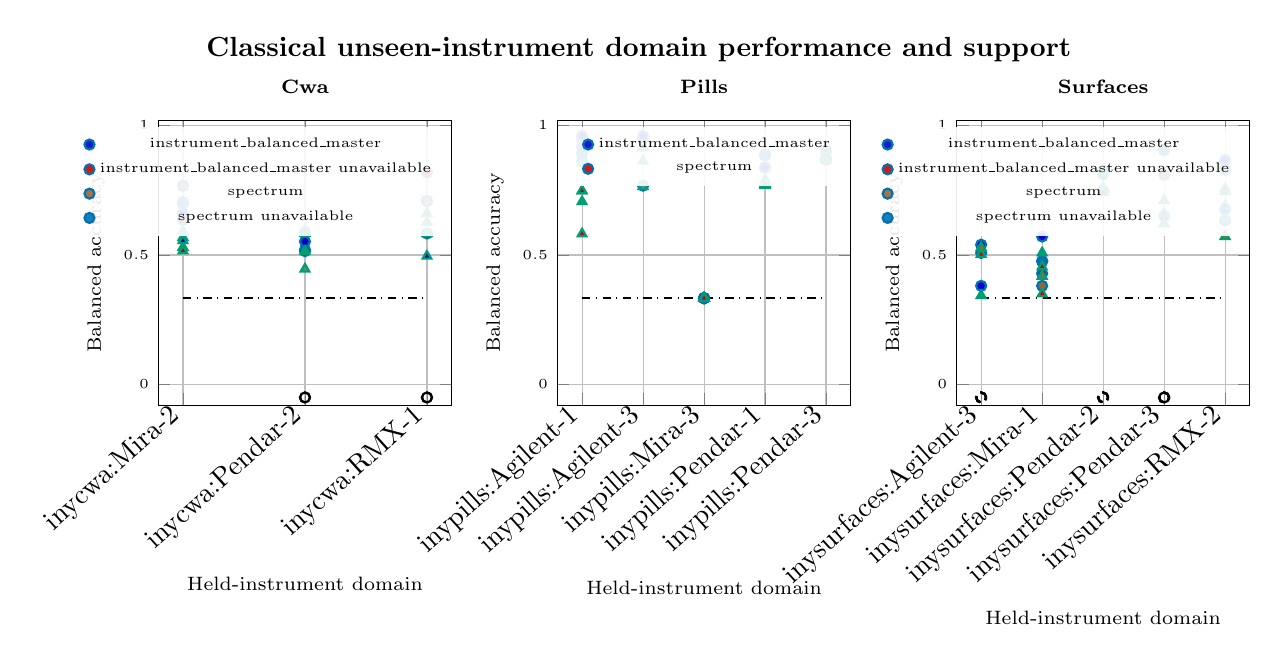
\begin{tikzpicture}
\begin{groupplot}[group style={group size=3 by 1, horizontal sep=1.35cm, vertical sep=1.5cm}, width=5.30cm, height=5.2cm, grid=major, tick label style={font=\tiny}, label style={font=\scriptsize}, title style={font=\scriptsize\bfseries,align=center}, legend style={font=\tiny,draw=none,fill=white,fill opacity=0.9,text opacity=1}]
\nextgroupplot[title={Cwa},xlabel={Held-instrument domain},ylabel={Balanced accuracy},ymin=-0.08,ymax=1.02,xtick={0,1,2},xticklabels={cwa:Mira-2,cwa:Pendar-2,cwa:RMX-1},x tick label style={rotate=42,anchor=east,font=	iny}]
\addplot+[color=atlas0,mark=*,mark size=1.8pt,line width=0.8pt,only marks] coordinates {(0,0.70436508) (1,0.51984127) (2,0.70833333)};
\addlegendentry{instrument\_balanced\_master}
\addplot+[color=atlas0,mark=*,mark size=1.8pt,line width=0.8pt,only marks] coordinates {(0,0.63624339) (1,0.51521164) (2,0.81944444)};
\addplot+[color=atlas0,mark=*,mark size=1.8pt,line width=0.8pt,only marks] coordinates {(0,0.76719577) (2,0.70833333)};
\addplot+[color=atlas0,mark=*,mark size=1.8pt,line width=0.8pt,only marks] coordinates {(0,0.6984127) (1,0.58796296) (2,0.58333333)};
\addplot+[color=atlas0,mark=*,mark size=1.8pt,line width=0.8pt,only marks] coordinates {(0,0.66137566) (1,0.55224868)};
\addplot+[color=atlas7,mark=o,mark size=1.8pt,line width=0.8pt,only marks,mark=o,mark options={draw=black,fill=atlas7}] coordinates {(1,-0.05)};
\addlegendentry{instrument\_balanced\_master unavailable}
\addplot+[color=atlas7,mark=o,mark size=1.8pt,line width=0.8pt,only marks,mark=o,mark options={draw=black,fill=atlas7}] coordinates {(2,-0.05)};
\addplot+[color=atlas2,mark=triangle*,mark size=1.8pt,line width=0.8pt,only marks] coordinates {(0,0.59206349) (1,0.44603175) (2,0.5830303)};
\addlegendentry{spectrum}
\addplot+[color=atlas2,mark=triangle*,mark size=1.8pt,line width=0.8pt,only marks] coordinates {(0,0.53015873) (1,0.51492063) (2,0.62666667)};
\addplot+[color=atlas2,mark=triangle*,mark size=1.8pt,line width=0.8pt,only marks] coordinates {(0,0.56785714) (2,0.66060606)};
\addplot+[color=atlas2,mark=triangle*,mark size=1.8pt,line width=0.8pt,only marks] coordinates {(0,0.55555556) (1,0.58391534) (2,0.49575758)};
\addplot+[color=atlas2,mark=triangle*,mark size=1.8pt,line width=0.8pt,only marks] coordinates {(0,0.51626984) (1,0.59724868)};
\addplot+[color=atlas7,mark=o,mark size=1.8pt,line width=0.8pt,only marks,mark=o,mark options={draw=black,fill=atlas7}] coordinates {(1,-0.05)};
\addlegendentry{spectrum unavailable}
\addplot+[color=atlas7,mark=o,mark size=1.8pt,line width=0.8pt,only marks,mark=o,mark options={draw=black,fill=atlas7}] coordinates {(2,-0.05)};
\addplot[black,dashdotted,line width=0.7pt,forget plot] coordinates {(0,0.33333333) (2,0.33333333)};
\nextgroupplot[title={Pills},xlabel={Held-instrument domain},ylabel={Balanced accuracy},ymin=-0.08,ymax=1.02,xtick={0,1,2,3,4},xticklabels={pills:Agilent-1,pills:Agilent-3,pills:Mira-3,pills:Pendar-1,pills:Pendar-3},x tick label style={rotate=42,anchor=east,font=	iny}]
\addplot+[color=atlas0,mark=*,mark size=1.8pt,line width=0.8pt,only marks] coordinates {(0,0.86111111) (1,0.95833333) (2,0.33333333) (3,0.88571429) (4,0.86904762)};
\addlegendentry{instrument\_balanced\_master}
\addplot+[color=atlas0,mark=*,mark size=1.8pt,line width=0.8pt,only marks] coordinates {(0,0.91666667) (1,0.95238095) (2,0.33333333) (3,0.83809524) (4,0.86904762)};
\addplot+[color=atlas0,mark=*,mark size=1.8pt,line width=0.8pt,only marks] coordinates {(0,0.94444444) (1,0.76785714) (2,0.33333333) (3,0.88571429) (4,0.86904762)};
\addplot+[color=atlas0,mark=*,mark size=1.8pt,line width=0.8pt,only marks] coordinates {(0,0.89166667) (1,0.95238095) (2,0.33333333) (3,0.88571429) (4,0.86904762)};
\addplot+[color=atlas0,mark=*,mark size=1.8pt,line width=0.8pt,only marks] coordinates {(0,0.95833333) (1,0.95833333) (2,0.33333333) (3,0.83809524) (4,0.9047619)};
\addplot+[color=atlas2,mark=triangle*,mark size=1.8pt,line width=0.8pt,only marks] coordinates {(0,0.58181818) (1,0.91375291) (2,0.33333333) (3,0.76884921) (4,0.86904762)};
\addlegendentry{spectrum}
\addplot+[color=atlas2,mark=triangle*,mark size=1.8pt,line width=0.8pt,only marks] coordinates {(0,0.74772727) (1,0.86247086) (2,0.33333333) (3,0.77414021) (4,0.86904762)};
\addplot+[color=atlas2,mark=triangle*,mark size=1.8pt,line width=0.8pt,only marks] coordinates {(0,0.85606061) (1,0.76456876) (2,0.33333333) (3,0.77414021) (4,0.86904762)};
\addplot+[color=atlas2,mark=triangle*,mark size=1.8pt,line width=0.8pt,only marks] coordinates {(0,0.70606061) (1,0.91375291) (2,0.33333333) (3,0.79001323) (4,0.86904762)};
\addplot+[color=atlas2,mark=triangle*,mark size=1.8pt,line width=0.8pt,only marks] coordinates {(0,0.74772727) (1,0.91841492) (2,0.33333333) (3,0.77414021) (4,0.9047619)};
\addplot[black,dashdotted,line width=0.7pt,forget plot] coordinates {(0,0.33333333) (4,0.33333333)};
\nextgroupplot[title={Surfaces},xlabel={Held-instrument domain},ylabel={Balanced accuracy},ymin=-0.08,ymax=1.02,xtick={0,1,2,3,4},xticklabels={surfaces:Agilent-3,surfaces:Mira-1,surfaces:Pendar-2,surfaces:Pendar-3,surfaces:RMX-2},x tick label style={rotate=42,anchor=east,font=	iny}]
\addplot+[color=atlas0,mark=*,mark size=1.8pt,line width=0.8pt,only marks] coordinates {(0,0.53968254) (1,0.47619048) (2,0.81212121) (4,0.86666667)};
\addlegendentry{instrument\_balanced\_master}
\addplot+[color=atlas0,mark=*,mark size=1.8pt,line width=0.8pt,only marks] coordinates {(1,0.42857143) (2,0.74848485) (4,0.82962963)};
\addplot+[color=atlas0,mark=*,mark size=1.8pt,line width=0.8pt,only marks] coordinates {(1,0.38095238) (3,0.80952381) (4,0.82962963)};
\addplot+[color=atlas0,mark=*,mark size=1.8pt,line width=0.8pt,only marks] coordinates {(0,0.50793651) (1,0.47619048) (3,0.9047619) (4,0.63333333)};
\addplot+[color=atlas0,mark=*,mark size=1.8pt,line width=0.8pt,only marks] coordinates {(0,0.38095238) (1,0.57142857) (2,0.82575758) (3,0.65079365) (4,0.67592593)};
\addplot+[color=atlas7,mark=o,mark size=1.8pt,line width=0.8pt,only marks,mark=o,mark options={draw=black,fill=atlas7}] coordinates {(3,-0.05)};
\addlegendentry{instrument\_balanced\_master unavailable}
\addplot+[color=atlas7,mark=o,mark size=1.8pt,line width=0.8pt,only marks,mark=o,mark options={draw=black,fill=atlas7}] coordinates {(0,-0.05) (3,-0.05)};
\addplot+[color=atlas7,mark=o,mark size=1.8pt,line width=0.8pt,only marks,mark=o,mark options={draw=black,fill=atlas7}] coordinates {(0,-0.05) (2,-0.05)};
\addplot+[color=atlas7,mark=o,mark size=1.8pt,line width=0.8pt,only marks,mark=o,mark options={draw=black,fill=atlas7}] coordinates {(2,-0.05)};
\addplot+[color=atlas2,mark=triangle*,mark size=1.8pt,line width=0.8pt,only marks] coordinates {(0,0.5026455) (1,0.45454545) (2,0.75909091) (4,0.74568966)};
\addlegendentry{spectrum}
\addplot+[color=atlas2,mark=triangle*,mark size=1.8pt,line width=0.8pt,only marks] coordinates {(1,0.41750842) (2,0.74242424) (4,0.6901341)};
\addplot+[color=atlas2,mark=triangle*,mark size=1.8pt,line width=0.8pt,only marks] coordinates {(1,0.35016835) (3,0.66111111) (4,0.7552682)};
\addplot+[color=atlas2,mark=triangle*,mark size=1.8pt,line width=0.8pt,only marks] coordinates {(0,0.52910053) (1,0.41750842) (3,0.71031746) (4,0.57183908)};
\addplot+[color=atlas2,mark=triangle*,mark size=1.8pt,line width=0.8pt,only marks] coordinates {(0,0.34391534) (1,0.50841751) (2,0.81666667) (3,0.62103175) (4,0.63697318)};
\addplot+[color=atlas7,mark=o,mark size=1.8pt,line width=0.8pt,only marks,mark=o,mark options={draw=black,fill=atlas7}] coordinates {(3,-0.05)};
\addlegendentry{spectrum unavailable}
\addplot+[color=atlas7,mark=o,mark size=1.8pt,line width=0.8pt,only marks,mark=o,mark options={draw=black,fill=atlas7}] coordinates {(0,-0.05) (3,-0.05)};
\addplot+[color=atlas7,mark=o,mark size=1.8pt,line width=0.8pt,only marks,mark=o,mark options={draw=black,fill=atlas7}] coordinates {(0,-0.05) (2,-0.05)};
\addplot+[color=atlas7,mark=o,mark size=1.8pt,line width=0.8pt,only marks,mark=o,mark options={draw=black,fill=atlas7}] coordinates {(2,-0.05)};
\addplot[black,dashdotted,line width=0.7pt,forget plot] coordinates {(0,0.33333333) (4,0.33333333)};
\end{groupplot}
\node[font=\normalsize\bfseries,anchor=south] at (current bounding box.north) {Classical unseen-instrument domain performance and support};
\end{tikzpicture}
\end{document}
